\phantomsection

\ifbool{latexml}{
 \chapter*{Important Formulas}
}{
 \addcontentsline{toc}{chapter}{Important Formulas}
}

% todo Tim - do we want to include derivative of an inverse?  would want three others
% (g(x))^n ? ln(f(x)) ? e^(f(x)) ?
\subsection{Differentiation Rules}

\bgroup
\footnotesize
\renewcommand{\arraystretch}{2.5}%
\setlength{\columnsep}{6pt}%
\noindent\lxAddClass{columns4}%
\hspace{-1.5em}%
\parbox{.29\linewidth}{% too narrow: 28
\begin{enumerate}
\item $\dfrac\dd{\dd x}(cx)=c$
\item $\dfrac\dd{\dd x}(u\pm v)=u'\pm v'$
\item $\dfrac\dd{\dd x}(u\cdot v)=uv'+u'v$%\qquad\null
\item $\dfrac\dd{\dd x}\left(\dfrac uv\right)=\dfrac{vu'-uv'}{v^2}$
\item $\dfrac\dd{\dd x}(u(v))=u'(v)v'$
\item $\dfrac\dd{\dd x}(f^{-1}(x))=\dfrac1{\fp(f^{-1}(x))}$
\item $\dfrac\dd{\dd x}(c)=0$
\item $\dfrac\dd{\dd x}(x)=1$
\item $\dfrac\dd{\dd x}(x^n)=nx^{n-1}$
\item $\dfrac\dd{\dd x}((f(x))^n)=n(f(x))^{n-1}\fp(x)$
\end{enumerate}}\hfill
\parbox{.23\linewidth}{% too narrow: 22, wide enough: 23
\begin{enumerate}\setcounter{enumi}{10}
\item $\dfrac\dd{\dd x}(e^x)=e^x$
\item $\dfrac\dd{\dd x}(e^{f(x)})=e^{f(x)}\fp(x)$
\item $\dfrac\dd{\dd x}(a^x)=\ln a\cdot a^x$
\item $\dfrac\dd{\dd x}(\ln x)=\frac1x$
\item $\dfrac\dd{\dd x}(\ln f(x))=\frac1{f(x)}\fp(x)$
\item $\dfrac\dd{\dd x}(\log_a x)=\frac1{x\ln a}$
\item $\dfrac\dd{\dd x}(\sin x)=\cos x$
\item $\dfrac\dd{\dd x}(\cos x)=-\sin x$
\item $\dfrac\dd{\dd x}(\csc x)=-\csc x\cot x$%\qquad\null
\item $\dfrac\dd{\dd x}(\sec x)=\sec x\tan x$
\end{enumerate}}\hfill
\parbox{.22\linewidth}{% too narrow: 21, wide enough: 22
\begin{enumerate}\setcounter{enumi}{20}
\item $\dfrac\dd{\dd x}(\tan x)=\sec^2x$
\item $\dfrac\dd{\dd x}(\cot x)=-\csc^2x$
\item $\dfrac\dd{\dd x}(\sin^{-1}x)=\frac1{\sqrt{1-x^2}}$
\item $\dfrac\dd{\dd x}(\cos^{-1}x)=\frac{-1}{\sqrt{1-x^2}}$
\item $\dfrac\dd{\dd x}(\csc^{-1}x)=\frac{-1}{\abs{x}\sqrt{x^2-1}}$
\item $\dfrac\dd{\dd x}(\sec^{-1}x)=\frac1{\abs{x}\sqrt{x^2-1}}$%\qquad\null
\item $\dfrac\dd{\dd x}(\tan^{-1}x)=\frac1{1+x^2}$
\item $\dfrac\dd{\dd x}(\cot^{-1}x)=\frac{-1}{1+x^2}$
\item $\dfrac\dd{\dd x}(\cosh x)=\sinh x$
\item $\dfrac\dd{\dd x}(\sinh x)=\cosh x$
\end{enumerate}}\hfill
\parbox{.25\linewidth}{% too narrow: 24, wide enough: 25
\begin{enumerate}\setcounter{enumi}{30}
\item $\dfrac\dd{\dd x}(\tanh x)=\sech^2x$
\item $\dfrac\dd{\dd x}(\sech x)=-\sech x\tanh x$
\item $\dfrac\dd{\dd x}(\csch x)=-\csch x\coth x$
\item $\dfrac\dd{\dd x}(\coth x)=-\csch^2 x$
\item $\dfrac\dd{\dd x}(\cosh^{-1}x)=\frac1{\sqrt{x^2-1}}$
\item $\dfrac\dd{\dd x}(\sinh^{-1}x)=\frac1{\sqrt{x^2+1}}$
\item $\dfrac\dd{\dd x}(\sech^{-1}x)=\frac{-1}{x\sqrt{1-x^2}}$
\item $\dfrac\dd{\dd x}(\csch^{-1}x)=\frac{-1}{\abs{x}\sqrt{1+x^2}}$
\item $\dfrac\dd{\dd x}(\tanh^{-1}x)=\frac1{1-x^2}$
\item $\dfrac\dd{\dd x}(\coth^{-1}x)=\frac1{1-x^2}$
\end{enumerate}}

\vfill

\subsection{Integration Rules}

\newcommand{\intRuleStrut}{\vphantom{\dfrac1{\sqrt{x^2}}}}%
\noindent\lxAddClass{columns3}%
\hspace{-1.5em}%
\parbox[t]{.37\linewidth}{% too narrow: 36
\begin{enumerate}
\item $\intRuleStrut\ds\int c\cdot f(x)\dd x=c\int f(x)\dd x$
\item $\intRuleStrut\ds\int\left(f(x)\pm g(x)\right)\dd x=\int f(x)\dd x\pm\int g(x)\dd x$
\item $\intRuleStrut\ds\int f(x)g'(x)\dd x=f(x)g(x)-\int\fp(x)g(x)\dd x$
\item $\intRuleStrut\ds\int f(g(x))g'(x)\dd x=\int f(u)\dd u$;\quad $u=g(x)$
\item $\intRuleStrut\ds\int0\dd x=C$
\item $\intRuleStrut\ds\int1\dd x=x+C$
\item $\intRuleStrut\ds\int x^n\dd x=\frac1{n+1}x^{n+1}+C;\quad n\ne-1$
\item $\intRuleStrut\ds\int e^x\dd x=e^x+C$
\item $\intRuleStrut\ds\int a^x\dd x=\frac1{\ln a}\cdot a^x+C$
\item $\intRuleStrut\ds\int\ln x\dd x=x\ln x-x+C$
\item $\intRuleStrut\ds\int\frac1x\dd x=\ln \abs{x} + C$
\item $\intRuleStrut\ds\int\cos x\dd x=\sin x+C$
\item $\intRuleStrut\ds\int\sin x\dd x=-\cos x+C$
\item $\intRuleStrut\ds\int\tan x\dd x=-\ln \abs{\cos x}+C$
\item $\intRuleStrut\ds\int\sec x\dd x=\ln \abs{\sec x+\tan x}+C$
\item $\intRuleStrut\ds\int\csc x\dd x=-\ln \abs{\csc x+\cot x}+C$
\end{enumerate}}%
\hfill
\begin{minipage}[t]{.6\linewidth}
\parbox[t]{.42\linewidth}{%
\begin{enumerate}\setcounter{enumi}{16}
\item $\intRuleStrut\ds\int\cot x\dd x=\ln \abs{\sin x}+C$
\item $\intRuleStrut\ds\int\sec^2 x\dd x=\tan x+C$
\item $\intRuleStrut\ds\int\csc^2x\dd x=-\cot x+C$
\item $\intRuleStrut\ds\int\sec x\tan x\dd x=\sec x+C$
\item $\intRuleStrut\ds\int\csc x\cot x\dd x=-\csc x+C$
\item $\intRuleStrut\ds\int\cos^2x\dd x=\frac x2+\frac{\sin(2x)}4+C$
\item $\intRuleStrut\ds\int\sin^2x\dd x=\frac x2-\frac{\sin(2x)}4+C$
\end{enumerate}}\hfill
\parbox[t]{.5\linewidth}{%
\begin{enumerate}\setcounter{enumi}{23}
\item $\intRuleStrut\ds\int\frac1{x^2+a^2}\dd x=\frac1a\tan^{-1}\frac xa+C$
\item $\intRuleStrut\ds\int\frac1{\sqrt{a^2-x^2}}\dd x=\sin^{-1}\frac x{\abs a}+C$
\item $\intRuleStrut\ds\int\frac1{x\sqrt{x^2-a^2}}\dd x=\frac1{\abs a}\sec^{-1}\abs{\frac  xa}+C$
\item $\intRuleStrut\ds\int\cosh x\dd x=\sinh x+C$
\item $\intRuleStrut\ds\int\sinh x\dd x=\cosh x+C$
\item $\intRuleStrut\ds\int\tanh x\dd x=\ln(\cosh x)+C$
\item $\intRuleStrut\ds\int\coth x\dd x=\ln\abs{\sinh x}+C$
\\$\intRuleStrut$
\end{enumerate}}%
\begin{enumerate}\setcounter{enumi}{30}
\item $\intRuleStrut\ds\int\sec^3 x\dd x=\frac12(\sec x\tan x+\ln\abs{\sec x+\tan x})+C$
\item\label{intRuleRtSmSq} $\intRuleStrut\ds\int\sqrt{x^2+a^2}\dd x=\frac x2\sqrt{x^2+a^2}+\frac{a^2}2\ln\left(x+\sqrt{x^2+a^2}\right)+C$
\item $\intRuleStrut\ds\int\frac1{\sqrt{x^2-a^2}}\dd x=\cosh^{-1}\frac xa+C=\ln\left(x+\sqrt{x^2-a^2}\right)+C$;\qquad $0<a<x$
\item $\intRuleStrut\ds\int\frac1{\sqrt{x^2+a^2}}\dd x=\sinh^{-1}\frac xa+C=\ln\left(x+\sqrt{x^2+a^2}\right)+C$;\qquad $0<a$
\item {$\intRuleStrut\ds\int\frac1{a^2-x^2}\dd x=\begin{cases}
\frac1a\tanh^{-1}\frac xa+C,&\abs x<\abs a\\
\frac1a\coth^{-1}\frac xa+C,&\abs a<\abs x
\end{cases}
\quad=\frac1{2a}\ln\abs{\frac{a+x}{a-x}}+C$}
\item $\intRuleStrut\ds\int\frac1{x\sqrt{a^2-x^2}}\dd x=-\frac1a\sech^{-1}\frac{\abs x}a+C=\frac1a\ln\abs{\frac x{a+\sqrt{a^2-x^2}}}+C$;\quad $0<\abs x<a$
\item $\ds\int\frac1{x\sqrt{x^2+a^2}}\dd x=-\frac1a\csch^{-1}\frac{\abs x}a+C=
\frac1a\ln\abs{\frac{x}{a+\sqrt{a^2+x^2}}}
%-\frac1a\ln\left(\frac ax+\frac{\sqrt{x^2+a^2}}{a\abs x}\right)
+C$;\quad $x\ne0$, $a>0$
\end{enumerate}
\end{minipage}
\egroup

%\normalsize

\clearpage

\noindent%
\begin{minipage}[t]{.53\linewidth}
\subsection{The Unit Circle}\vspace{-2\baselineskip}

\pdftooltip{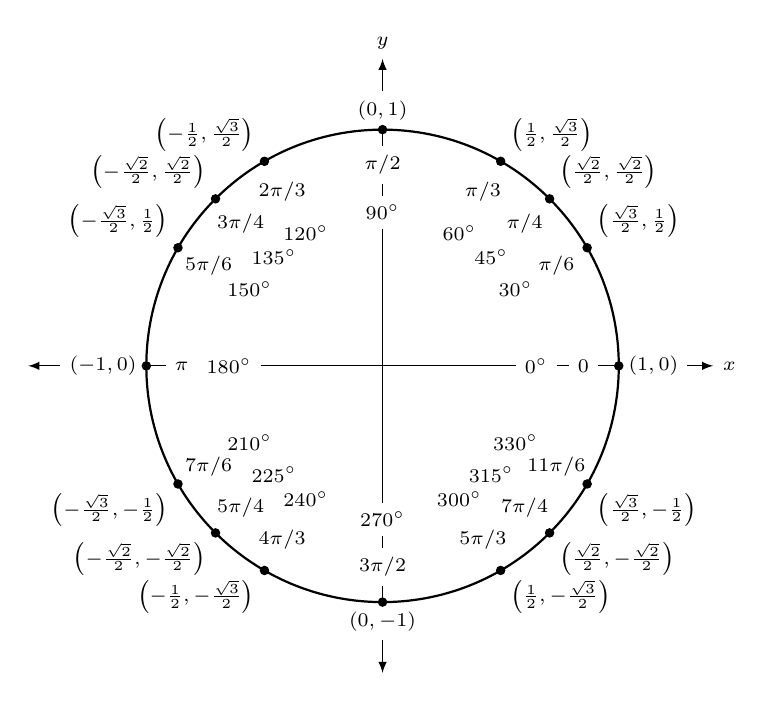
\begin{tikzpicture}[scale=3]
\draw [<->,>=latex] (-1.5,0) -- (1.4,0) node [right] {\scriptsize $x$};
\draw [<->,>=latex] (0,-1.3) -- (0,1.3) node [above] {\scriptsize $y$};
\foreach \x / \y / \z / \w / \v in {
	0/0/{1,0}/right/white,
	30/{\pi/6}/{\frac{\sqrt{3}}2,\frac 12}/above right/none,%
	45/{\pi/4}/{\frac{\sqrt{2}}2,\frac{\sqrt{2}}2}/above right/none,
	60/{\pi/3}/{\frac{1}2,\frac{\sqrt{3}}2}/{above right}/none,
	90/ {\pi/2}/{0,1}/above/white,%
	120/{2\pi/3}/{-\frac{1}2,\frac{\sqrt{3}}2}/above left/none, 
	135/{3\pi/4}/{-\frac{\sqrt{2}}2,\frac{\sqrt{2}}2}/above left/none, 
	150/ {5\pi/6}/{-\frac{\sqrt{3}}2,\frac{1}2}/above left/none,%
	180/ {\pi}/{-1,0}/left/white, 
	210/{7\pi/6}/{-\frac{\sqrt{3}}2,-\frac{1}2}/below left/none, 
	225/{5\pi/4}/{-\frac{\sqrt{2}}2,-\frac{\sqrt{2}}2}/below left/none, 
	240/{4\pi/3}/{-\frac{1}2,-\frac{\sqrt{3}}2}/below left/none,
	270/{3\pi/2}/{0,-1}/below/white, 
	300/{5\pi/3}/{\frac{1}2,-\frac{\sqrt{3}}2}/below right/none, 
	315/{7\pi/4}/{\frac{\sqrt{2}}2,-\frac{\sqrt{2}}2}/below right/none, 
	330/{11\pi/6}/{\frac{\sqrt{3}}2,-\frac{1}2}/below right/none%
}
{%
	\draw (\x:.65cm) node [fill=\v] {\scriptsize \x$^\circ$};
	\draw (\x:.85cm) node [fill=\v] {\scriptsize $\y$};
	\draw (\x:1cm) node [\w,fill=\v] {\scriptsize $\left(\z\right)$};
	\draw [fill=black] (\x:1) circle (.5pt);
}
\draw [thick] (0,0) circle (1);
\end{tikzpicture}}{ALT-TEXT-TO-BE-DETERMINED}
\end{minipage}%
%
\begin{minipage}[t]{.45\linewidth}
\subsection{Definitions of the Trigonometric Functions}

\noindent%
\small
%\begin{minipage}[t]{.48\linewidth}
\subsubsection*{Unit Circle Definition}\vspace{-2\baselineskip}
%\textbf{\normalsize Unit Circle Definition}

\noindent%
\begin{minipage}{.4\linewidth}
\small
\begin{align*}
\sin\theta &= y & \cos\theta &= x \\
\csc\theta &= \dfrac1y & \sec\theta &= \dfrac1x \\
\tan\theta &= \frac yx & \cot\theta &= \frac xy
\end{align*}
\end{minipage}\hfill
\begin{minipage}{.56\linewidth}
\centering
\pdftooltip{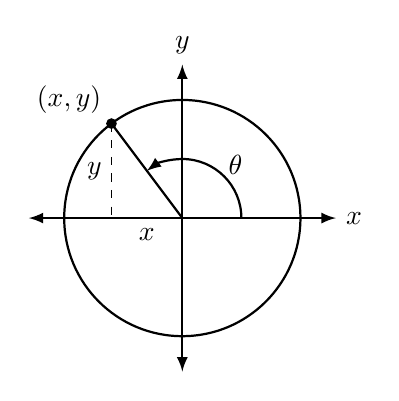
\begin{tikzpicture}[>=latex,scale=1.5,thick]
\draw [<->](-1.3,0)--(1.3,0) node [right] {$x$};
\draw [<->] (0,-1.3) -- (0,1.3) node [above] {$y$};
\draw (0,0) circle (1);
\draw [fill= black] (-.6,.8) circle (1pt);
\draw (0,0) -- (-.6,.8) node [above left] {$(x,y)$};
\draw [->] (.5,0) arc (0:127:.5);
\draw [dashed,thin] (-.6,.8) -- (-.6,0) node [pos=.5,left] {$y$};
\draw (-.3,0) node [below] {$x$};
\draw (.45,.45) node {$\theta$};
\end{tikzpicture}}{ALT-TEXT-TO-BE-DETERMINED}
\end{minipage}\vspace{-2\baselineskip}

\subsubsection*{Right Triangle Definition}

\noindent%
\begin{minipage}{.56\linewidth}
 \centering
 \pdftooltip{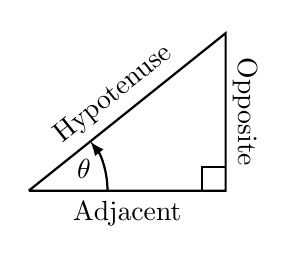
\begin{tikzpicture}[thick]
  \draw (0,0) -- (2.5,0) node [below,pos=.5] {Adjacent} -- (2.5,2) node [pos=.5,rotate=-90,shift={(0pt,7pt)}] {Opposite} -- (0,0) node [pos=.5,above,rotate=38.7] {Hypotenuse} node [shift={(20pt,8pt)}] {$\theta$};
  \draw[->,>=latex] (1,0) arc (0:38.7:1);
  \draw (2.2,0) -- (2.2,.3) -- (2.5,.3);
 \end{tikzpicture}}{ALT-TEXT-TO-BE-DETERMINED}
\end{minipage}%
\begin{minipage}{.4\linewidth}
 \small
 \begin{align*}
  \sin\theta &= \frac{\text{O}}{\text{H}} & \csc\theta &= \frac{\text{H}}{\text{O}} \\
  \cos\theta &= \frac{\text{A}}{\text{H}} & \sec\theta &= \frac{\text{H}}{\text{A}} \\
  \tan\theta &= \frac{\text{O}}{\text{A}} & \cot\theta &= \frac{\text{A}}{\text{O}}
 \end{align*}
\end{minipage}
\end{minipage}

\vfill

\subsection{Common Trigonometric Identities}

\noindent%
\begin{minipage}[t]{.25\linewidth}
	\subsubsection*{Pythagorean~Identities}\vspace{-\baselineskip}
	\begin{align*}
		\sin ^2x+\cos ^2x= 1 \\
		\tan^2x+ 1 = \sec^2 x \\
		1 + \cot^2x=\csc^2 x
	\end{align*}
\end{minipage}%
\begin{minipage}[t]{.43\linewidth}
	\subsubsection*{Cofunction Identities}\vspace{-\baselineskip}
	\begin{align*}
		\sin(\tfrac{\pi}{2}-x) &= \cos x &
		\csc(\tfrac{\pi}{2}-x) &= \sec x \\
		\cos(\tfrac{\pi}{2}-x) &= \sin x &
		\sec(\tfrac{\pi}{2}-x) &= \csc x \\
		\tan(\tfrac{\pi}{2}-x) &= \cot x &
		\cot(\tfrac{\pi}{2}-x) &= \tan x
	\end{align*}
\end{minipage}%
\begin{minipage}[t]{.32\linewidth}
\subsubsection*{Even/Odd Identities}\vspace{-\baselineskip}
\begin{align*}
\sin(-x) &= -\sin x &
\csc(-x) &= -\csc x \\
\cos(-x) &= \phantom{-}\cos x &
\sec(-x) &= \phantom{-}\sec x \\
\tan(-x) &= -\tan x &
\cot(-x) &= -\cot x
\end{align*}
\end{minipage}

\vfill

\noindent%
\begin{minipage}[t]{.44\linewidth}
\subsubsection*{Sum to Product Formulas}\vspace{-\baselineskip}
\begin{align*}
\sin x+\sin y &= 2\sin (\tfrac{x+y}2)\cos(\tfrac{x-y}2) &~\\
\sin x-\sin y &= 2\sin (\tfrac{x-y}2)\cos(\tfrac{x+y}2) \\
\cos x+\cos y &= 2\cos (\tfrac{x+y}2)\cos(\tfrac{x-y}2) \\
\cos x-\cos y &= 2\sin (\tfrac{x+y}2)\sin(\tfrac{y-x}2)
\end{align*}
\end{minipage}%
\begin{minipage}[t]{.3\linewidth}
\subsubsection*{Power-Reducing Formulas}\vspace{-\baselineskip}
\begin{align*}
\sin^2 x &= \frac{1-\cos 2x}{2} & \vphantom{\left(\frac11\right)}&~\\
\cos^2 x &= \frac{1+\cos 2x}{2} & \vphantom{\left(\frac11\right)}\\
\tan^2 x &= \frac{1-\cos 2x}{1+\cos 2x}
\end{align*}
\end{minipage}%
\begin{minipage}[t]{.25\linewidth}
	\subsubsection*{Double Angle Formulas}\vspace{-\baselineskip}
	\begin{align*}
		\sin 2x &= 2\sin x\cos x &~\\
		\cos 2x &= \cos^2x - \sin^2 x \\
		&= 2\cos^2x-1 \\
		&= 1-2\sin^2x \\
		\tan 2x &= \frac{2\tan x}{1-\tan^2 x}
	\end{align*}
\end{minipage}

\vfill

\noindent
\begin{minipage}[t]{.45\linewidth}
\subsubsection*{Product to Sum Formulas}\vspace{-\baselineskip}
\begin{align*}
\sin x\sin y &= \tfrac12\bigl(\cos(x-y)-\cos(x+y)\bigr) &~\\
\cos x\cos y &= \tfrac12\bigl(\cos(x-y)+\cos(x+y)\bigr) \\
\sin x\cos y &= \tfrac12\bigl(\sin(x+y)+\sin(x-y)\bigr)
\end{align*}
\end{minipage}%
\begin{minipage}[t]{.45\linewidth}
\subsubsection*{Angle Sum/Difference Formulas}\vspace{-\baselineskip}
\begin{align*}
\sin (x\pm y) &= \sin x\cos y \pm \cos x\sin y &~\\
\cos (x\pm y) &= \cos x\cos y \mp \sin x\sin y\\
\tan (x\pm y) &= \frac{\tan x\pm \tan y}{1\mp \tan x\tan y}
\end{align*}
\end{minipage}

\vfill

\subsection*{Domains and ranges of inverse trigonometric functions}\vspace{-.5\baselineskip}
\tagpdfsetup{table/header-rows={1}}
\begin{tabular}{ccc @{\hspace{3em}} ccc}
Inverse Function & Domain & Range &
Inverse Function & Domain & Range \\\midrule
$\sin^{-1}x$ & $[-1,1]$ & $[-\pi/2,\pi/2]$ & % ([
$\csc^{-1}x$ & $(-\infty,-1]\cup[1,\infty)$ & $[-\pi/2,0)\cup(0,\pi/2]$ \\ % )]
$\cos^{-1}x$ & $[-1,1]$ & $[0,\pi]$ & % ([
$\sec^{-1}x$ & $(-\infty,-1]\cup[1,\infty)$ & $[0,\pi/2)\cup(\pi/2,\pi]$ \\ % )]
$\tan^{-1}x$ & $(-\infty,\infty)$ & $(-\pi/2,\pi/2)$ &
$\cot^{-1}x$ & $(-\infty,\infty)$ & $(0,\pi)$
\end{tabular}

\clearpage

%\mbox{}\vfill

\subsection{Areas and Volumes}

%\vfill

\bgroup
\renewcommand{\arraystretch}{5}
%\renewcommand{\baselinestretch}{1.5}
\renewcommand{\cellwidth}{\ifbool{latexml}{.4}{}\linewidth}
\tagpdfsetup{table/tagging=presentation}
\begin{tabular}{
	p{.22\linewidth}p{.2\linewidth} @{\hskip 4em}
	p{.22\linewidth}p{.2\linewidth}
}
	\parbox[t]{\cellwidth}{%
		\textbf{Triangles}\\
		$h=a\sin\theta$\\
		Area ${}=\frac12bh$ \\
		Law of Cosines: \\
		$c^2=a^2+b^2-2ab\cos\theta$%
	}
	&
	\pdftooltip{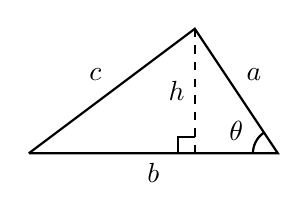
\begin{tikzpicture}[x=30pt,y=30pt,thick,baseline={(current bounding box.north)}]
		\draw (0,0) -- node [below]  { $b$} (3,0) node [shift={(-15pt,8pt)}] {$\theta$} -- node [above right] { $a$} (2,1.5) -- node [above left] { $c$} (0,0);
		\draw (2.7,0) arc (180:125:.3);
		\draw [dashed] (2,1.5) -- (2,0) node [pos=.5,left] {$h$};
		\draw (2,.2) -- (1.8,.2) -- (1.8,0);
	\end{tikzpicture}}{ALT-TEXT-TO-BE-DETERMINED}
	&
	\parbox[t]{\cellwidth}{%
		\textbf{Right Circular Cone}\\
		Volume ${} = \frac 13 \pi r^2h $\\
		Surface Area = \\
		$\pi r\sqrt{r^2+h^2} +\pi r^2$%
	}
	&
	\pdftooltip{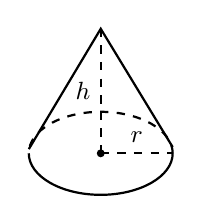
\begin{tikzpicture}[x=13pt,y=15pt,thick,
				baseline={(current bounding box.north)}]
		\begin{scope}[xscale=2]
			\draw (-1,0) arc (-180:0:1);
			\draw [dashed] (1,0) arc (0:180:1);
		\end{scope}
		\draw (-2,.1) -- (0,3) -- (2,.15);
		\draw [dashed] (0,3) -- node [left] {\small $h$} (0,0);
		\draw [dashed] (0,0) -- node [above] {\small $r$} (2,0);
		\draw [fill=black] (0,0) circle (1pt);
	\end{tikzpicture}}{ALT-TEXT-TO-BE-DETERMINED}
	\\
	\parbox[t]{\cellwidth}{%
		\textbf{Parallelograms}\\
		Area ${} = bh$%
	}
	&
	\pdftooltip{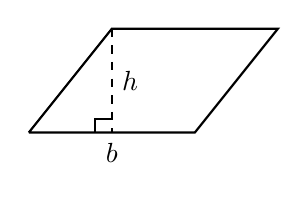
\begin{tikzpicture}[x=30pt,y=25pt,thick,
				baseline={(current bounding box.north)}]
		\draw (0,0) -- node [below]  { $b$} (2,0) -- (3,1.5) -- (1,1.5) -- (0,0);
		\draw [dashed] (1,1.5) -- node [right] {$h$} (1,0);
		\draw (.8,0) -- (.8,.2) -- (1,.2);
	\end{tikzpicture}}{ALT-TEXT-TO-BE-DETERMINED}
	&
	\parbox[t]{\cellwidth}{%
		\textbf{Right Circular Cylinder}\\
		Volume ${} = \pi r^2h $\\
		Surface Area = \\
		$2\pi rh  +2\pi r^2$%
	}
	&
	\pdftooltip{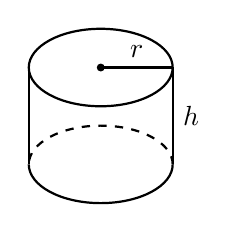
\begin{tikzpicture}[x=13pt,y=14pt,thick,
				baseline={(current bounding box.north)}]
		\begin{scope}[xscale=2]
			\draw (-1,0) arc (-180:0:1);
			\draw [dashed] (1,0) arc (0:180:1);
		\end{scope}
		\draw (0,2.5) ellipse [x radius=2,y radius=1];
		\draw (-2,0) -- (-2,2.5) (2,0) -- node [right] {$h$} (2,2.5);
		\draw (0,2.5) -- node [above] {$r$} (2,2.5);
		\draw [fill=black] (0,2.5) circle (1pt);
	\end{tikzpicture}}{ALT-TEXT-TO-BE-DETERMINED}
	\\
	\parbox[t]{\cellwidth}{%
		\textbf{Trapezoids}\\
		Area ${} = \frac12(a+b)h $%
	}
	&
	\pdftooltip{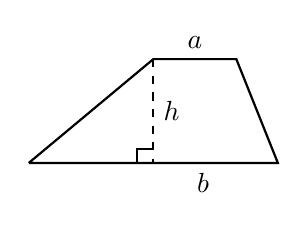
\begin{tikzpicture}[x=30pt,y=25pt,thick,
				baseline={(current bounding box.north)}]
		\draw (0,0) -- node [below,pos=.7]  { $b$} (3,0) -- (2.5,1.5) -- node [above] {$a$} (1.5,1.5) -- (0,0);
		\draw [dashed] (1.5,1.5) -- node [right] {$h$} (1.5,0);
		\draw (1.3,0) -- (1.3,.2) -- (1.5,.2);
	\end{tikzpicture}}{ALT-TEXT-TO-BE-DETERMINED}
	&
	\parbox[t]{\cellwidth}{%
		\textbf{Sphere}\\
		Volume ${} = \frac43\pi r^3 $\\
		Surface Area ${} = 4\pi r^2$%
	}
	&
	\pdftooltip{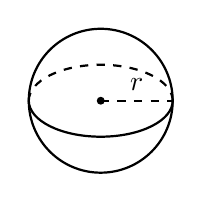
\begin{tikzpicture}[x=13pt,y=13pt,thick,
				baseline={(current bounding box.north)}]
		\begin{scope}[xscale=2]
			\draw (-1,0) arc (-180:0:1);
			\draw [dashed] (1,0) arc (0:180:1);
		\end{scope}
		\draw (0,0) circle (2);
		\draw [dashed] (0,0) -- node [above] {$r$} (2,0);
		\draw [fill=black] (0,0) circle (1pt);
	\end{tikzpicture}}{ALT-TEXT-TO-BE-DETERMINED}
	\\
	\parbox[t]{\cellwidth}{%
		\textbf{Circles}\\
		Area ${} = \pi r^2 $\\
		Circumference ${} = 2\pi r$%
	}
	&
	\pdftooltip{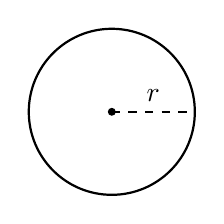
\begin{tikzpicture}[x=30pt,y=30pt,thick,
				baseline={(current bounding box.north)}]
		\draw (0,0) circle (1);
		\draw [dashed] (0,0) -- node [above] {$r$} (1,0);
		\draw [fill=black] (0,0) circle (1pt);
	\end{tikzpicture}}{ALT-TEXT-TO-BE-DETERMINED}
	&
	\parbox[t]{\cellwidth}{%
		\textbf{General Cone}\\
		Area of Base ${} = A $\\
		Volume ${} = \frac13Ah$%
	}
	&
	\pdftooltip{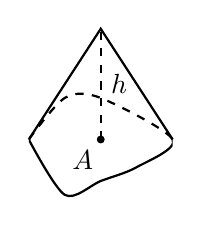
\begin{tikzpicture}[x=13pt,y=10pt,thick,
				baseline={(current bounding box.north)}]
		\begin{scope}
			\clip (0,0) rectangle (4,-2.5);
			\draw [smooth] plot coordinates {(0,0) (1,1.5) (2,1.5) (4,0) (3,-1) (2,-1.5) (1,-2) (0,0)};
		\end{scope}
		\begin{scope}
			\clip (0,0) rectangle (4,2.5);
			\draw [smooth,dashed] plot coordinates {(0,0) (1,1.5) (2,1.5) (4,0) (3,-1) (2,-1.5) (1,-2) (0,0)};
		\end{scope}
		\draw (0,0) -- (2,4) -- (4,0);
		\draw [dashed] (2,0) -- node [right] {$h$}(2,4);
		\draw [fill=black] (2,0) circle (1pt);
		\draw (1.5,-.75) node {$A$};
	\end{tikzpicture}}{ALT-TEXT-TO-BE-DETERMINED}
	\\
	\parbox[t]{\cellwidth}{%
		\textbf{Sectors of Circles}\\
		$\theta$ in radians \\
		Area ${} = \frac12\theta r^2$ \\
		$s=r\theta$%
	}
	&
	\pdftooltip{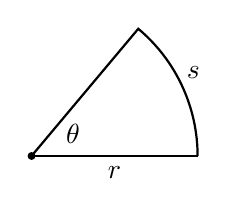
\begin{tikzpicture}[x=30pt,y=30pt,thick,
				baseline={(current bounding box.north)}]
		\draw (2,0) arc (0:50:2) -- (0,0);
		\draw [] (0,0) -- node [below] {$r$} (2,0);
		\draw [fill=black] (0,0) circle (1pt);
		\draw (1.95,1.0) node {$s$};
		\draw (0,0) node [shift={(15pt,8pt)}] {$\theta$};
	\end{tikzpicture}}{ALT-TEXT-TO-BE-DETERMINED}
	&
	\parbox[t]{\cellwidth}{%
		\textbf{General Right Cylinder}\\
		Area of Base ${} = A $\\
		Volume ${} = Ah$%
	}
	&
	\pdftooltip{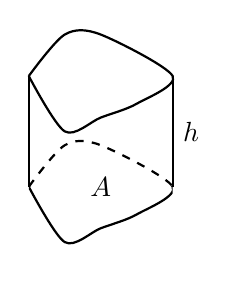
\begin{tikzpicture}[x=13pt,y=10pt,thick,
				baseline={(current bounding box.north)}]
		\begin{scope}
			\clip (0,0) rectangle (4,-2.5);
			\draw [smooth] plot coordinates {(0,0) (1,1.5) (2,1.5) (4,0) (3,-1) (2,-1.5) (1,-2) (0,0)};
		\end{scope}
		\begin{scope}
			\clip (0,0) rectangle (4,2.5);
			\draw [smooth,dashed] plot coordinates {(0,0) (1,1.5) (2,1.5) (4,0) (3,-1) (2,-1.5) (1,-2) (0,0)};
		\end{scope}
		\begin{scope}[shift={(0,4)}]
			\draw [smooth] plot coordinates {(0,0) (1,1.5) (2,1.5) (4,0) (3,-1) (2,-1.5) (1,-2) (0,0)};
		\end{scope}
		\draw (0,0) -- (0,4) (4,0) -- (4,4) node [pos=.5,right] {$h$};
		\draw (2,0) node {$A$};
	\end{tikzpicture}}{ALT-TEXT-TO-BE-DETERMINED}
\end{tabular}
\egroup

\clearpage

\subsection{Algebra}

\subsubsection*{Factors and Zeros of Polynomials}
Let $p(x) = a_n x^n + a_{n-1} x^{n-1} + \dots + a_1 x + a_0$ be a polynomial.  If $p(a)=0$, then $a$ is a $zero$ of the polynomial and a solution
of the equation $p(x)=0$.  Furthermore, $(x-a)$ is a $factor$ of the polynomial.

\vfill

\subsubsection*{Fundamental Theorem of Algebra}
An $n$th degree polynomial has $n$ (not necessarily distinct) zeros.  Although all of these zeros may be imaginary, a real polynomial of odd degree
must have at least one real zero.

\vfill

\subsubsection*{Quadratic Formula}
If $p(x) = ax^2 + bx + c$, %and $0 \le b^2 - 4ac$,
then the zeros of $p$ are $x=\dfrac{-b\pm \sqrt{b^2-4ac}}{2a}$

\vfill

\subsubsection*{Special Factoring}\vspace{-\baselineskip}
\begin{flalign*}
x^2 - a^2 &= (x-a)(x+a)
&
x^3 \pm a^3 &= (x\pm a)(x^2\mp ax+a^2)
&
x^4 - a^4 &= (x^2-a^2)(x^2+a^2)
\end{flalign*}

\vfill

\subsubsection*{Binomial Theorem}\vspace{-\baselineskip}
\begin{align*}
(x+y)^2 &= x^2 + 2xy + y^2 &
(x+y)^3 &= x^3 + 3x^2y + 3xy^2 + y^3 \\
(x+y)^4 &= x^4 + 4x^3y + 6x^2y^2 + 4xy^3 + y^4 &
(x+y)^n &=\sum_{k=0}^n \binom{n}{k}x\primeskip^{n-k}y\primeskip^k
\end{align*}

\vfill

\subsubsection*{Rational Zero Theorem}
If $p(x) = a_n x^n + a_{n-1} x^{n-1} + \dotsb + a_1 x + a_0$ has integer coefficients, then every $rational$ $zero$ of $p$ is of the form
$x=r/s$, where $r$ is a factor of $a_0$ and $s$ is a factor of $a_n$.

\vfill

\subsubsection*{Factoring by Grouping}
$ac x^3 + ad x^2 + bcx + bd = ax^2(cx+d)+b(cx+d)=(ax^2+b)(cx+d)$

\vfill

\subsubsection*{Arithmetic Operations}\vspace{-\baselineskip}
\begin{align*}
&ab+ac=a(b+c) && \frac{a}{b}+\frac{c}{d} = \frac{ad+bc}{bd} && \frac{a+b}{c} = \frac{a}{c} + \frac{b}{c} \\[.3\baselineskip]
&\frac{\left(\dfrac{a\vphantom{d}}{b}\right)}{\left(\dfrac{c}{d}\right)}=\left(\frac{a}{b}\right)\left(\frac{d}{c}\right)=\frac{ad}{bc} 
&& \frac{\left(\dfrac{a}{b}\right)}{c} = \frac{a}{bc}
&& \frac{a}{\left(\dfrac{b}{c}\right)} = \frac{ac}{b} \\[.3\baselineskip]
&a\left(\frac{b}{c}\right)= \frac{ab}{c} && \frac{a-b}{c-d}=\frac{b-a}{d-c} && \frac{ab+ac}{a}=b+c
\end{align*}

\vfill

\subsubsection*{Exponents and Radicals}\vspace{-\baselineskip}
\begin{flalign*}
&a^0=1, \; \; a \ne 0 & (ab)^x&=a^xb^x & a^xa^y &= a^{x+y} & \sqrt{a}&=a^{1/2} & \frac{a^x}{a^y}&=a^{x-y} & \sqrt[n]{a}&=a^{1/n} \\
&\left(\frac{a}{b}\right)^x=\frac{a^x}{b^x} & \sqrt[n]{a^m}&=a^{m/n} & a^{-x}&=\frac{1}{a^x} & \sqrt[n]{ab}&=\sqrt[n]{a}\sqrt[n]{b} &
(a^x)^y&=a^{xy} & \sqrt[n]{\frac{a}{b}}&=\frac{\sqrt[n]{a}}{\sqrt[n]{b}}
\end{flalign*}

\clearpage

\subsection{Additional Formulas}

\vfill

\subsubsection*{Summation Formulas}\vspace{-\baselineskip}

\begin{align*}
\sum^n_{i=1}{c} &= cn
&
\sum^n_{i=1}{i} &= \frac{n(n+1)}{2}
&
\sum^n_{i=1}{i^2} &= \frac{n(n+1)(2n+1)}{6}
&
\sum^n_{i=1}{i^3} &= \left(\frac{n(n+1)}{2}\right)^2
\end{align*}

\vfill

\subsubsection*{Trapezoidal Rule}

\noindent$\ds\int_a^b{f(x)}\dd x \approx \frac{\Delta x}{2}\left[f(x_1)+2f(x_2) + 2f(x_3) + \dotsb + 2f(x_{n}) + f(x_{n+1})\right]$\smallskip\\
with  $\text{Error} \leq \dfrac{(b-a)^3}{12n^2}\left[ \max \abs{\fpp(x)}\right]$

\vfill

\subsubsection*{Simpson's Rule}

\noindent$\ds\int_a^b{f(x)}\dd x \approx \frac{\Delta x}{3}\left[f(x_1)+4f(x_2) + 2f(x_3) + 4f(x_4) + \dotsb + 2f(x_{n-1}) + 4f(x_{n}) + f(x_{n+1})\right] 
$\smallskip\\
with $\text{Error} \leq \dfrac{(b-a)^5}{180n^4}\left[ \max \abs{f\primeskip^{(4)}(x)}\right]$

\vfill

\subsubsection*{Arc Length}

\noindent
$\ds L = \int_a^b{\sqrt{1+ \fp(x)^2}}\dd x$

\vfill

% also add volume of revolution, or nothing at all
% \begin{minipage}[t]{.4\linewidth}
%  \subsection*{Surface of Revolution}
%  $\ds S = 2\pi \int_a^b{f(x) \sqrt{1+ f\,'(x)^2}}\dd x  $\smallskip\\
%  {\small (where $f(x)\geq 0$)}\medskip\\
%  $\ds S = 2\pi \int_a^b{x \sqrt{1+ f\,'(x)^2}}\dd x 
%  $\smallskip\\
%  {\small (where $a,b \geq 0$)}\bigskip\\~
% \end{minipage}

\noindent
\begin{minipage}[t]{.5\linewidth}
  \subsubsection*{Work Done by a Variable Force}
  $\ds W = \int_a^b{F(x)}\dd x$
\end{minipage}%
\begin{minipage}[t]{.5\linewidth}
 \subsubsection*{Force Exerted by a Fluid}
 $\ds F = \int_a^b{w\,d(y)\,\ell(y)}\dd y$
\end{minipage}

\vfill

\subsubsection*{Taylor Series Expansion for $f(x)$}
\noindent$\ds p_n(x) = f(c) + \fp(c)(x-c) + \frac{\fpp(c)}{2!}(x-c)^2 + \frac{f\,'''(c)}{3!}(x-c)^3 + \dotsb + \frac{f\,^{(n)}(c)}{n!}(x-c)^n + \dotsb $

\vfill

%\subsection*{Maclaurin Series Expansion for $f(x)$} %{, where $c=0$}
%\noindent$\ds p_n(x) = f(0) + \fp(0)x + \frac{\fpp(0)}{2!}x^2 + \frac{f\,'''(0)}{3!}x^3 + \dotsb + \frac{f\,^{(n)}(0)}{n!}x^n$ + \dotsb

\subsubsection*{Standard Form of Conic Sections}

{\addtolength{\tabcolsep}{6pt}
\tagpdfsetup{table/header-rows={1,2,3}}
\begin{tabular}{ c c c c c }
\multicolumn{2}{c}{Parabola} & \hspace{5em}Ellipse\hspace{5em} & \multicolumn{2}{c}{Hyperbola} \\
Vertical axis & Horizontal axis & & Foci and vertices & Foci and vertices \\
& & & on $x$-axis & on $y$-axis \\
$y=\dfrac{x^2}{4p}$ & $x=\dfrac{y^2}{4p}$ & $\dfrac{x^2}{a^2}+\dfrac{y^2}{b^2}=1$ & $\dfrac{x^2}{a^2}-\dfrac{y^2}{b^2}=1$ & $\dfrac{y^2}{b^2}-\dfrac{x^2}{a^2}=1$
\end{tabular}}

\clearpage

\subsection{Summary of Tests for Series}\label{tab_series_tests}

Notation: Infinite series $\ds\sum_{n=1}^\infty a_n$ with sequence of partial sums $\{S_n\}=\{a_1+a_2+a_3+\dots+a_n\}$

\begin{center}
\renewcommand{\arraystretch}{3.8}
\addtolength{\tabcolsep}{5pt}
\tagpdfsetup{table/header-rows={1}}
\begin{tabular}{ p{.7in} p{1.2in} @{} p{2.5in} p{1.6in} }

%\toprule% this leaves too much space afterward
\specialrule{\heavyrulewidth}{0pt}{-2ex}
\lxBeginTableHead
\centering Test & \centering Series & \centering Convergence or Divergence & \parbox[t]{\linewidth}{\centering Comment} \\\lxEndTableHead
\specialrule{\lightrulewidth}{0pt}{-2ex}
%\midrule% not quite as bad as the toprule, but still to much space

\parbox[t]{\linewidth}{\centering Definition of Series} & \parbox[t]{\linewidth}{\centering$\ds\sum_{n=1}^\infty a_n$} & \parbox[t]{\linewidth}{\centering series converges if and\\only if $\{S_n\}$ converges} & \parbox[t]{\linewidth}{\centering used when a formula\\for $S_n$ can be found}\\

\parbox[t]{\linewidth}{\centering Divergence Test} & \parbox[t]{\linewidth}{\centering$\ds\sum_{n=1}^\infty a_n$} & \parbox[t]{\linewidth}{\centering diverges if $\ds\lim_{n\to\infty}a_n\neq0$} & \parbox[t]{\linewidth}{\centering no conclusion if $\ds\lim_{n\to\infty}a_n=0$}\\

\parbox{\linewidth}{\centering Alternating Series} & \parbox[t]{\linewidth}{\centering $\ds\pm\sum_{n=1}^\infty (-1)^n b_n$} & \parbox{\linewidth}{\centering converges if $b_n>0$, $\{b_n\}$ is\\decreasing, and $\ds\lim_{n\to\infty}b_n=0$} & \parbox{\linewidth}{\centering check that conditions hold eventually; no information about divergence} \\

\parbox{\linewidth}{\centering Geometric Series} & \parbox[t]{\linewidth}{\centering$\ds\sum_{n=0}^\infty ar\primeskip^n$} & \parbox{\linewidth}{\centering converges if and\\only if $\abs r<1$} & \parbox[t]{\linewidth}{\centering Sum $=\dfrac a{1-r}$} \\

\parbox{\linewidth}{\centering Telescoping Series} & \parbox[t]{\linewidth}{\centering$\ds\sum_{n=1}^\infty b_n-b_{n+m}$} & \parbox{\linewidth}{\centering converges if and only\\if $\{S_n\}$ converges} & \parbox{\linewidth}{\centering most terms of $S_n$\\subtract away} \\

\parbox[t]{\linewidth}{\centering$p$-Series} & \parbox[t]{\linewidth}{\centering$\ds\sum_{n=1}^\infty\frac1{(an+b)^p}$} & \parbox{\linewidth}{\centering converges if and\\only if $p>1$} & \parbox[t]{\linewidth}{\centering assumes $an+b\ne0$} \\

\parbox{\linewidth}{\centering$p$-Series For Logarithms} & \parbox[t]{\linewidth}{\centering$\ds\sum_{n=1}^\infty\frac1{(an+b)(\log n)^p}$} & \parbox{\linewidth}{\centering converges if and\\only if $p>1$} & \parbox{\linewidth}{\centering logarithm's base doesn't affect convergence.} \\

\parbox[t]{\linewidth}{\centering Integral Test} & \parbox[t]{\linewidth}{\centering$\ds\sum_{n=1}^\infty a_n$} & \parbox{\linewidth}{\centering converges if and only if\\$\ds\int_k^\infty a(n)\dd n$ converges} & \parbox{\linewidth}{\centering $a_n = a(n)$ must be positive and decreasing eventually} \\

\parbox[t]{\linewidth}{\centering Direct Comparison} & \parbox[t]{\linewidth}{\centering$\ds\sum_{n=1}^\infty a_n$, $\ds\sum_{n=1}^\infty b_n$ $0<a_n\le b_n$} & \parbox[t]{\linewidth}{\centering $\sum b_n\text{ converges }\Rightarrow\sum a_n$ converges $\sum a_n\text{ diverges }\Rightarrow\sum b_n$ diverges} & \parbox[t]{\linewidth}{\centering consider geometric\\or $p$-series} \\\addlinespace

\parbox[t]{\linewidth}{\centering Limit Comparison} & \parbox[t]{\linewidth}{\centering$\ds\sum_{n=1}^\infty a_n$, $\ds\sum_{n=1}^\infty b_n$ $0<a_n,b_n$} & \parbox{\linewidth}{\centering if $\ds\lim_{n\to\infty} a_n/b_n=L$\\ $L>0$: both converge or diverge together\\ $L=0$: $\sum b_n\text{ converges }\Rightarrow\sum a_n$ converges\\$L=\infty$: $\sum b_n\text{ diverges }\Rightarrow\sum a_n$ diverges} & \parbox[t]{\linewidth}{\centering consider geometric\\or $p$-series} \\\addlinespace

\parbox[t]{\linewidth}{\centering Ratio/Root Test} & \parbox[t]{\linewidth}{\centering$\ds\sum_{n=1}^\infty a_n$} & \parbox[t]{\linewidth}{\centering$L=\begin{cases}
\ds\lim_{n\to\infty}\abs{a_{n+1}/a_n}&\text{Ratio Test} \\
%\ds\lim_{n\to\infty}\abs{\frac{a_{n+1}}{a_n}}&\text{Ratio Test} \\
\ds\lim_{n\to\infty}\abs{a_n}^{1/n}&\text{Root Test}
\end{cases}$\\
$L<1$: converges\\
$L>1$ or $L=\infty$: diverges\\
$L=1$: test indeterminate}
& \parbox[t]{\linewidth}{\vskip-1.3\baselineskip\relax\centering use Ratio Test for products, factorials, or powers in terms\\\medskip use Root Test for series of the form $a_n=(b_n)^n$} \\\addlinespace \bottomrule

\end{tabular}

\end{center}

\textbf{Absolute convergence:} $\ds\sum_{n=1}^\infty\abs{a_n}$ converges (and by \emph{Absolute Convergence Theorem}, $\ds\sum_{n=1}^\infty a_n$ converges)

\textbf{Conditional convergence:} $\ds\sum_{n=1}^\infty a_n$ converges but $\ds\sum_{n=1}^\infty\abs{a_n}$ diverges

% trying to avoid an underfull hbox?
